\section{Sets}
\subsection{Sets and Subsets}

A \textbf{set} is a collection of objects. Objects in a set are called \textbf{elements}.
Order does \underline{not} matter, and there are \underline{no} duplicates.

Roster notation:
\begin{align*}
  A & = \{2, 4, 6, 10\} \\
  B & = \{4, 6, 10, 2\} \\
  A & = B
\end{align*}

To show membership, use the $\in$ symbol. For example, $2 \in A$, while $7 \not \in A$.
The empty set, which contains nothing, typically uses the $\emptyset$ symbol, or \{\}.
Sets can be finite, or infinite. \textbf{Cardinality} of a set is the number of elements in a set.
For example, the cardinality of A is 4.
\begin{align*}
  \left\lvert A\right\rvert = 4
\end{align*}
Cardinality can be infinite. Consider the set of all the integers, $\mathbb{Z}$. $\left\lvert \mathbb{Z}\right\rvert = \infty$

\begin{align*}
  \mathbb{N} & : \text{ set of natural numbers}                                         & \mathbb{Z} & : \text{ set of integers}                        \\
             & = \{0, 1, 2, 3, \ldots\}                                                 &            & = \{\ldots, -2, -1, 0, 1, 2, \ldots\}            \\
  \\
  \mathbb{B} & : \text{ set of rational numbers}                                        & \mathbb{R} & : \text{ set of real numbers}                    \\
             & = \{x | x = \frac{a}{b} \text{ where } a, b \in \mathbb{Z}, b \not = 0\} &            & = \{x | x \text{ has a decimal representation}\} \\
\end{align*}

The subset operator is $\subseteq$
\begin{align*}
  A         & \subseteq B \text{  if } \forall x (x \in A \implies x \in B) \\
  A         & \subseteq A \text{  is true for \underline{any} set}          \\
  \emptyset & \subseteq A \text{ is true for \underline{any} set}
\end{align*}

Sometimes it is easier to define a set by defining properties that all the elements have.
That is easy to do in \textbf{set builder notation}.
\begin{align*}
  A & = \{x \in S: A(x)\}, \text{ where $S$ is another set}                \\
  C & = \{x \in \mathbb{Z}: 0 < x < 100 \text{ and } x \text{ is prime}\}. \\
  D & = \{x \in \mathbb{R}: \left\lvert x\right\rvert < 1\}
\end{align*}

The \textbf{Universal Set}, usually called 'U', is a set that contains all elements mentioned in a particular context.
For example, a discussion about certain types of real numbers, it would be understood that any element in the discussion
is a real number. Sets are often represented pictorially with \textbf{Venn Diagrams}.

\begin{center}
  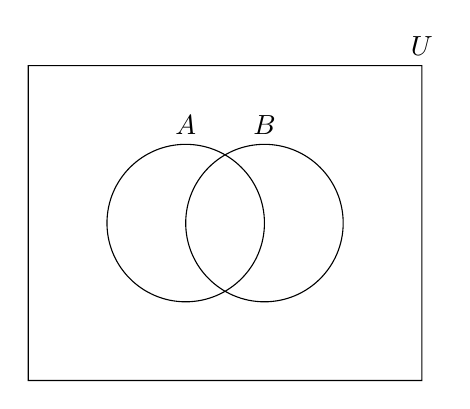
\begin{tikzpicture}[fill=white]
    \draw (0,0) circle (1) (0,1)  node [text=black,above] {$A$}
    (1,0) circle (1) (1,1)  node [text=black,above] {$B$}
    (-2,-2) rectangle (3,2) node [text=black,above] {$U$};
  \end{tikzpicture}
\end{center}

If $A \subseteq B$ and there is an element of $B$ that is not an element of $A$, meaning $A \not = B$,
then $A$ is a \textbf{proper subset} of $B$, denoted as $A \subset B$. An important fact is that
$\mathbb{N} \subset \mathbb{Z} \subset \mathbb{B} \subset \mathbb{R}$

\subsection{Sets of sets}

Elements of sets can be sets themselves, consider $A = \{\{1, 2\}, \emptyset, \{1, 2, 3\}, \{1\}\}$.
The cardinality of $A$ is 4, $\left\lvert A\right\rvert = 4$. Additionally, $\{1, 2\} \in A$, but
$1 \not \in A$.

The \textbf{Powerset} of A, denoted as $P(A)$ is the set of all subsets of $A$. For example,
\begin{align*}
  A    & = \{1, 2, 3\}                                                        \\
  P(A) & = \{\{1\}, \{2\}, \{3\}, \{1, 2\}, \{1, 3\}, \{2, 3\}, \{1, 2, 3\}\}
\end{align*}

\subsubsection{Cardinality of a Powerset}

Let A be a finite set of cardinality $n$. Then the cardinality of the powerset of A is $2^n$.
\begin{align*}
  \left\lvert A\right\rvert    & = n   \\
  \left\lvert P(A)\right\rvert & = 2^n
\end{align*}

\subsection{Union and Intersection}

\textbf{Intersection} set operation: $\cap$.
$A$ intersected with $B$ is defined to be the set containing elements which are in both $A$ \underline{and} $B$.
That is, $A \cap B = \{x: x \in A \land x \in B\}$.
\begin{center}
  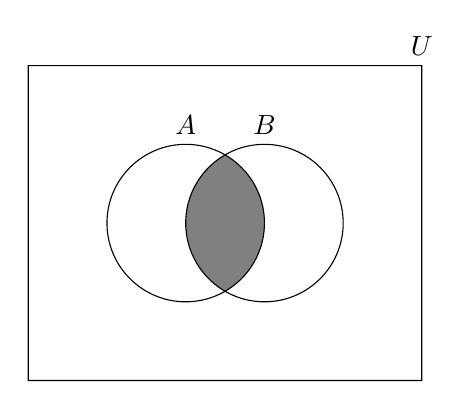
\begin{tikzpicture}
    \filldraw[fill=white] (-2,-2) rectangle (3,2);
    \scope % A \cap B
    \clip (0,0) circle (1);
    \fill[gray] (1,0) circle (1);
    \endscope
    % outline
    \draw (0,0) circle (1) (0,1)  node [text=black,above] {$A$}
    (1,0) circle (1) (1,1)  node [text=black,above] {$B$}
    (-2,-2) rectangle (3,2) node [text=black,above] {$U$};
  \end{tikzpicture}
\end{center}

Intersection $\cap$ can also apply to infinite sets:
\begin{align*}
  A        & =\{x \in \mathbb{Z}: x \text{ is an integer multiple of 2}\}  \\
  B        & =\{x \in \mathbb{Z}: x \text{ is an integer multiple of 3}\}  \\
  A \cap B & = \{x \in \mathbb{Z}: x \text{ is an integer multiple of 6}\}
\end{align*}

\noindent \textbf{Union} set operation $\cup$.
$A$ union with $B$ is defined to be the set containing elements which are in $A$ \underline{or} $B$.
That is, $A \cup B = \{x: x \in A \lor x \in B\}$.
\begin{center}
  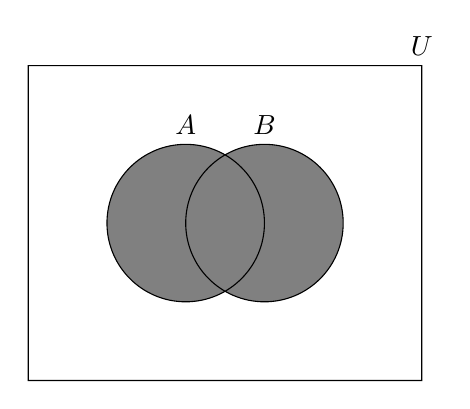
\begin{tikzpicture}
    \filldraw[fill=white] (-2,-2) rectangle (3,2);
    \fill[gray] (0,0) circle (1);
    \fill[gray] (1,0) circle (1);
    % outline
    \draw (0,0) circle (1) (0,1)  node [text=black,above] {$A$}
    (1,0) circle (1) (1,1)  node [text=black,above] {$B$}
    (-2,-2) rectangle (3,2) node [text=black,above] {$U$};
  \end{tikzpicture}
\end{center}

A special notation, similar to $\sum$ or $\prod$ notation, allows for compound representation of the
intersections or unions of a long sequence of sets.
\begin{align*}
  \bigcap_{i=1}^{n} A_{i} & = A_1 \cap A_2 \cap A_3 \cap \cdots \cap A_n = \{x : x \in A, \text{ for \underline{all} } 1 \leq i \leq n\}  \\
  \bigcup_{i=1}^{n} A_{i} & = A_1 \cup A_2 \cup A_3 \cup \cdots \cup A_n = \{x : x \in A, \text{ for \underline{some} } 1 \leq i \leq n\} \\
\end{align*}

Consider $A_j =$ a word with $j$ letters, with $U =$ is the Oxford English Dictionary.
\begin{align*}
  \bigcup_{j=1}^{10} A_j & = \text{ the set of all words with 10 letters or fewer in the OED} \\
  \bigcap_{j=1}^{45} A_j & = \emptyset                                                        \\
  \bigcup_{j=1}^{45} A_j & = \text{ the set of all words in the OED.}
\end{align*}

\subsection{More set operations}

\textbf{Difference} set operation $-$.
$A$ difference with $B$ is defined to be the set containing elements which are in $A$ but \underline{not} $B$.
That is, $A - B = \{x: x \in A \land x \not \in B\}$. A set difference is \underline{not} strictly commutative, often
$A - B \not = B - A$.
\begin{center}
  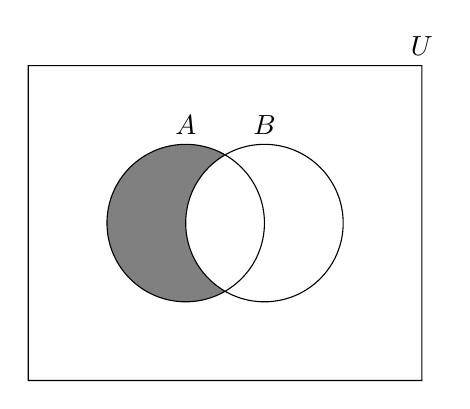
\begin{tikzpicture}[fill=gray]
    % left hand
    \scope
    \clip (-2,-2) rectangle (2,2)
    (1,0) circle (1);
    \fill (0,0) circle (1);
    \endscope
    % outline
    \draw (0,0) circle (1) (0,1)  node [text=black,above] {$A$}
    (1,0) circle (1) (1,1)  node [text=black,above] {$B$}
    (-2,-2) rectangle (3,2) node [text=black,above] {$U$};
  \end{tikzpicture}
\end{center}

\noindent \textbf{Symmetric Difference} set operation $\triangle$.
$A$ symmetric difference with $B$ is defined to be the set containing elements which are in $A$ or $B$, but not $A$ and $B$.
That is, $A \triangle B = \{x: x \in A \oplus  x \in B\}$.
\begin{center}
  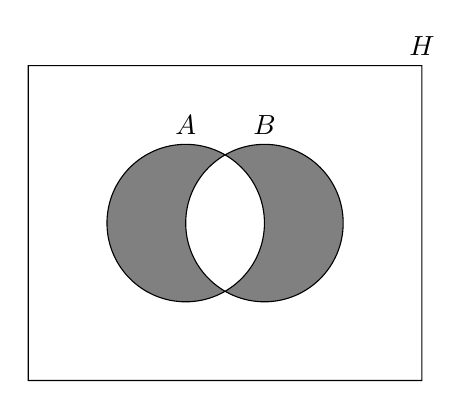
\begin{tikzpicture}[fill=gray]
    % left hand
    \scope
    \clip (-2,-2) rectangle (2,2)
    (1,0) circle (1);
    \fill (0,0) circle (1);
    \endscope
    % right hand
    \scope
    \clip (-2,-2) rectangle (2,2)
    (0,0) circle (1);
    \fill (1,0) circle (1);
    \endscope
    % outline
    \draw (0,0) circle (1) (0,1)  node [text=black,above] {$A$}
    (1,0) circle (1) (1,1)  node [text=black,above] {$B$}
    (-2,-2) rectangle (3,2) node [text=black,above] {$H$};
  \end{tikzpicture}
\end{center}

\noindent \textbf{Complement} set operation $\overline{ }$.
complement $A$ is defined to be the set containing elements in $U$ which are not in $A$.
That is, $\overline{A}= \{x: x \in U \land x \not \in A\}$.
\begin{center}
  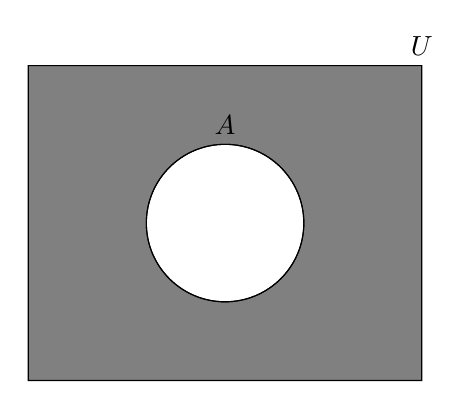
\begin{tikzpicture}[fill=white]
    \draw[fill=gray] (-2,-2) rectangle (3,2);
    \draw[fill=white] (0.5,0) circle (1);
    % outline
    \draw (0.5,0) circle (1) (0.5,1)  node [text=black,above] {$A$}
    (-2,-2) rectangle (3,2) node [text=black,above] {$U$};
  \end{tikzpicture}
\end{center}

\begin{center}
  \begin{tabular}{l|c|l}
    \multicolumn{3}{c}{\textbf{Summary of Set Operations}}                       \\
    Operation            & Notation        & Set Builder                         \\
    \hline
    Intersection         & $A \cap B$      & $\{x: x \in A \land x \in B\}$      \\
    Union                & $A \cup B$      & $\{x: x \in A \lor x \in B\}$       \\
    Difference           & $A - B$         & $\{x: x \in A \land x \not \in B\}$ \\
    Symmetric Difference & $A \triangle B$ & $\{x: x \in A \oplus  x \in B\}$    \\
    Complement           & $\overline{A}$  & $\{x: x \in U \land x \not \in A\}$ \\
  \end{tabular}
\end{center}

\subsection{Set identities}

The laws of propositional logic can be used to derive corresponding set identities.
A \textbf{set identity} is an equation involving sets that is true,
regardless of the contents of the sets used in the expression.
\begin{center}
  \begin{tabular}{r|c|c}
    \textbf{Law Name} & $\cup$ Union                                           & $\cap$ Intersection                                    \\
    \hline
    Idempotent        & $A \cup A = A$                                         & $A \cap A = A$                                         \\
    Associative       & $(A \cup B) \cup C = A \cup (B \cup C)$                & $(A \cap B) \cap C = A \cap (B \cap C)$                \\
    Commutative       & $A \cup B = B \cup A$                                  & $A \cap B = B \cap A$                                  \\
    Distributive      & $A \cup (B \cap C) = (A \cup B) \cap (A \cup C)$       & $A \cap (B \cup C) = (A \cap B) \cup (A \cap C)$       \\
    Identity          & $A \cup \emptyset = A$                                 & $A \cap U = A$                                         \\
    Domination        & $A \cup U = U$                                         & $A \cap \emptyset = \emptyset$                         \\
    Double Complement & $\overline{\overline{A}} = A$                                                                                   \\
    Complement        & $A \cup \overline{A} =$ T                              & $A \cap \overline{A} =$ F                              \\
    DeMorgan          & $\overline{A \cup B} = \overline{A} \cap \overline{B}$ & $\overline{A \cap B} = \overline{A} \cup \overline{B}$ \\
    Absorption        & $A \cup (A \cap B) = A$                                & $A \cap (A \cup B) = A$
  \end{tabular}
\end{center}

\subsection{Cartesian products}

An \textbf{ordered pair} of items is written $(x, y)$, where the first entry is $x$ and the second entry is $y$.
The use of $()$ instead of $\{\}$ indicates that order matters.

\noindent \textbf{Cartesian Product} of $A$ and $B$, $A \times B = \{(a, b) : a \in A \land b \in B\}$
\begin{align*}
  A & = \{1, 2\}    & A \times B & = \{(1, a), (1, b), (1, c), (2, a), (2, b), (2, c)\} \\
  B & = \{a, b, c\} & B \times A & = \{(a, 1), (a, 2), (b, 1), (b, 2), (c, 1), (c, 2)\}
\end{align*}

An ordered list of 3 items is called an \textbf{ordered triple}, denoted as $(x, y, z)$.
For a size of $\geq 4$, use the term \textbf{n-tuple}. For example, $(u, w, x, y, z)$.
\begin{align*}
  A_1 \times A_2 \times \cdots \times A_n = \{(a_1, a_2, \ldots, a_n) : a_i \in A \text{ for all $i$ such that} 1 \leq i \leq n\}
\end{align*}
Another Example
\begin{align*}
  A & = \{a, b\}          & (a, 1, y, \beta)  & \in A \times B \times C \times D      \\
  B & = \{1, 2\}          & (b, 1, x, \alpha) & \in A \times B \times C \times D      \\
  C & = \{x, y\}          & (1, b, x, \beta)  & \not \in A \times B \times C \times D \\
  D & = \{\alpha, \beta\} &                   & \text{order matters}
\end{align*}

$A \times A = A^2$, and in general,
\begin{align*}
  A^k = \underbrace{A \times A \times \cdots \times A}_{k-times}
\end{align*}
The \textbf{Cardinality of Cartesian Products}:
\begin{align*}
  \left\lvert A^n \right\rvert                           & = {\left\lvert A \right\rvert}^n                                               \\
  \left\lvert A_1 \times A_2 \times \cdots  \right\rvert & = \left\lvert A_1 \right\rvert \cdot \left\lvert A_2 \right\rvert \cdot \cdots
\end{align*}

\subsubsection{Strings}

A sequence of characters is called a \textbf{string}.
The set of characters used in a set of string is called the \textbf{alphabet} for the set of strings.
The \textbf{length} of a string is the number of characters in the string.
For example, the length of $'xxyxyx'$ is $6$.
The \textbf{empty string} is a string whose length is $0$, and is usually denoted by $\lambda$.
It is useful for $A^0$, for some alphabet $A$. $\{0, 1\}^0 = \{\lambda\}$.
If $s$ and $t$ are two strings, then the \textbf{concatenation} of $s$ and $t$ is the string obtained by putting $s$ and $t$ together.
\begin{align*}
  s & = 010 & st & = 01011 \\
  t & = 11  & t0 & = 110
\end{align*}
Strings are used to specify passwords for computers or online accounts.
Security systems vary with respect to the alphabet of characters allowed or required in a valid password.
Strings also play an important rules in discrete mathematics as a mathematical tool to help count cardinality of sets.

\subsection{Partitions}

Two sets, $A$ and $B$, are said to be \textbf{disjoint} if their intersection is empty $(A \cap B = \emptyset)$.
A sequence of sets, $A_1, A_2, A_3, \ldots, A_n$, is \textbf{pairwise disjoint} if every pair of distinct sets in the sequence is disjoint.
A \textbf{partition} of a non-empty set $A$ is a collection of non-empty subsets such that each element of $A$ is in exactly one of the subsets.
$A_1, A_2, A_3, \ldots, A_n$ is a partition for a nonempty set $A$ if:
\begin{itemize}
  \item For all $i, A_i \subseteq A$
  \item For all $i, A_i \not = \emptyset$
  \item $A_1, A_2, \ldots, A_n$ are pairwise disjoint
  \item $A = \bigcup_{i=1}^{n} A_i$, for some $n \in \mathbb{Z}^+$
\end{itemize}
\begin{center}
  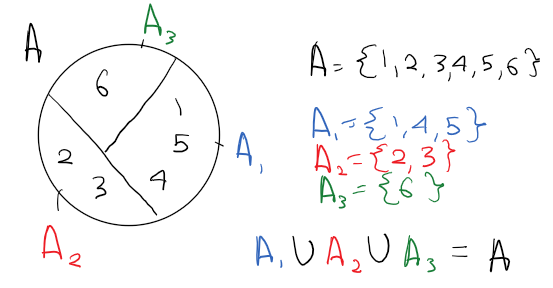
\includegraphics[width=.6\linewidth]{partitions.png}
\end{center}